
%------------------------------------------------

\section{Poisson distribution}
\label{exer:poisson_distr}

\subsection{Generate Poisson variables}

\begin{enumerate}
		\marginnote{Do not use any predefined method for the binomial and Poisson distribution.}
	\item Generate $n = 10$ uniformly distributed values of $t$ in $[0, \Delta t = 10^{3}]$.
	\item Compute the number of accepted events $k$ that happen in interval $[0, \delta t]$, with $\delta t = p \cdot \Delta t$ t and $p = 0.01$.
	\item Repeat $10^{5}$ times, and populate the histogram of $k$.
	\item Plot the histogram of $k$ and compare it with the theoretical binomial and Poisson distribution.
	\item Repeat for all combinations of: $n = \{ 10, 100, 1000 \}$ and $p = \{ 0.01, 0.05, 0.1, 0.5 \}$.
\end{enumerate}

(Figure~\ref{fig:Poisson_distr})

\begin{figure}
	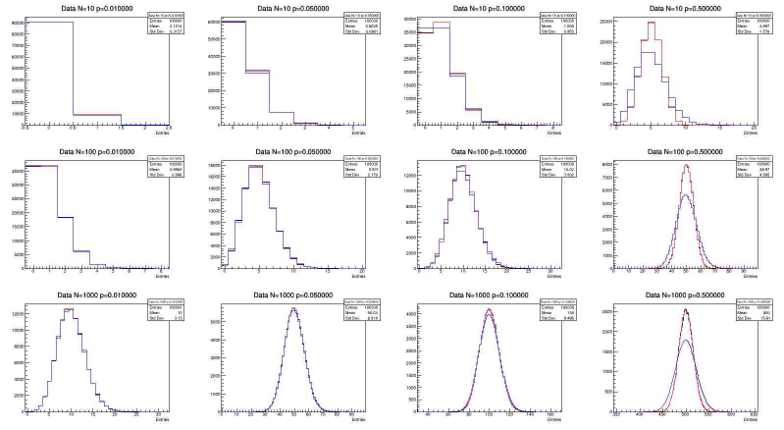
\includegraphics{exercise/Poisson_distr.png}
	\caption[Poisson distribution.][6pt]{Poisson distribution.}
	\label{fig:Poisson_distr}
\end{figure}

($\hookleftarrow$ \ref{subsec:poisson_distr})
